\begin{figure}[htb]
    \vspace{-0.1cm}
    \begin{center}
    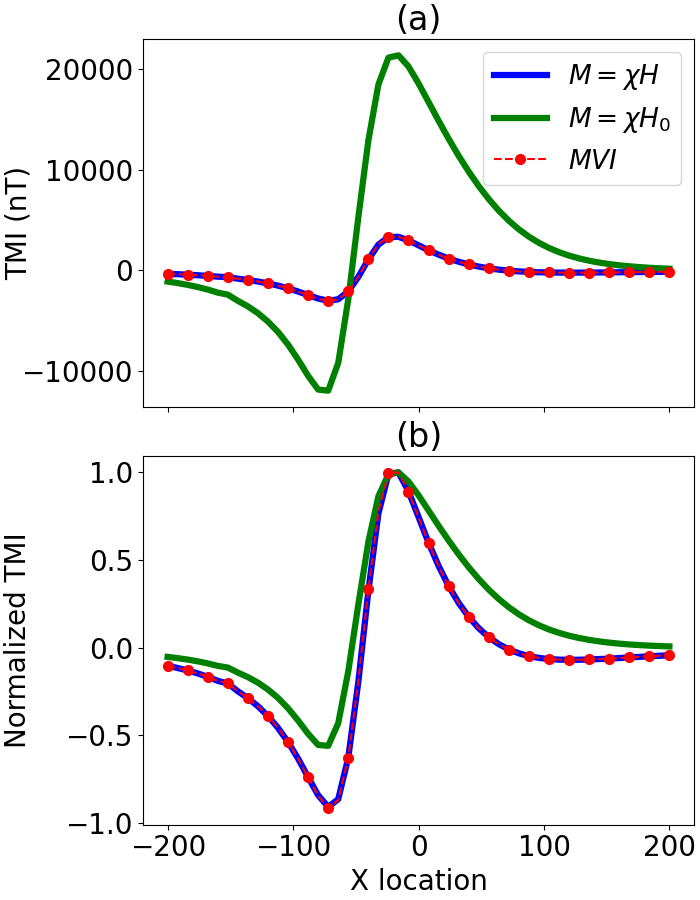
\includegraphics[width=\columnwidth]{figures/TMI.png}
    \end{center}
    \vspace{-0.5cm}
\caption{
    (a) Simulated TMI data running above the plate. The blue line is data accounting for demagnetization. The green line is data neglecting demagnetization. The red line is magnetic vector forward modeled data using the magnetization from the demagnetization corrected numerical solution.
    (b) The same data normalized by their respective maximum values.
}
\label{fig:TMI}
\vspace{-0.1cm}
\end{figure}
